\documentclass{article}
\usepackage[utf8]{inputenc}
\usepackage{amsmath, amssymb, amsthm}
\usepackage{graphicx, float}
\graphicspath{ {./imagens/} }
\usepackage{multicol}
\usepackage[brazil]{babel}
\usepackage{pgfplots}
\pgfplotsset{compat=1.18}
\usepackage[letterpaper, top = 1in, bottom = 1.0 in, left = 1.2 in, right = 1.2 in, heightrounded]{geometry}

%%%%%%%%%%%%%%%%%%%%%%%%% Caso haja dúvidas na Symbologia %%%%%%%%%%%%%%%%
% https://detexify.kirelabs.org/classify.html
%%%%%%%%%%%%%%%%%%%%%%%%% Parâmetros de construção %%%%%%%%%%%%%%%%%%%%%%%
\setlength{\parindent}{0pt}
\setlength{\parskip}{0.8em}

\title{\textbf{Repositório de Estatistica e Probabilidade}}
\author{UFSC Joinville - EMB5010 \\ Artur Gemaque}
\date{\today}
%%%%%%%%%%%%%%%%%%%%%%%%%% COMEÇO DO DOCUMENTO %%%%%%%%%%%%%%%%%%%%%%%%%%%
\begin{document}
\maketitle

\begin{abstract}
Este documento tempo como principal funcionalidade registrar os contudos ensinados 
em sala de aula pelo professor Jaimes, ademais servirá como fonte de estudo para as 
provas referentes há Matéria.
\end{abstract}

\begin{multicols}{2} % Início da seção com duas colunas
\section{ Medidas Descritivas:}

  \subsection{Valores de cálculo}
      Vamos começar com as definições mais simplórias da matéria que são resultado do cálculo dos dados.

      \subsubsection{Média}
      A média aritmética de um conjunto de n números é a soma desses números dividida por n.
        \begin{center}
          $ \overset{\_}{x} =  \overset{n}{\underset{i=1}{\sum}} \frac{X_i}{n}  $
        \end{center}

      \subsubsection{Variância}
      A variância é um conceito fundamental em estatística que mede a dispersão de um conjunto de dados em relação à sua média.
        \begin{center}
          $ (S)^2 =  \frac{\overset{n}{\underset{i=1}{\sum}} (X_i - \overset{\_}{x} )^2 }{n - 1} $
        \end{center}

      \subsubsection{Desvio padrão}
      O desvio padrão é uma medida de dispersão estatística que indica o quão afastados os 
      dados de um conjunto estão da sua média. Ele é a raiz quadrada da variância, o que o 
      torna mais interpretável.
        \begin{center}
          $ S = \sqrt[2]{S^2}$
        \end{center}

  \subsection{Valores de análise}
    Partindo agora para valores que são obtidos apartir dos dados ordenados em formato crescente. 
    Observação que as seguintes fórmulas serão para que possamos obter as posição dos referidos valores.    
    
    \subsubsection{Mediana}
    Mediana é o número no centro de um grupo de números.
    \begin{center}
      $ Md = X_{(\frac{n + 1}{2})} $
    \end{center}

    \subsubsection{Quartis}
    Os quartis são valores que dividem uma amostra de dados em quatro partes iguais e são usados para 
    avaliar a dispersão e a tendência central de um conjunto de dados. Eles são os valores contidos nas 
    posições de $ n*25\% $ entre outras porcentagens, caso "n" dê um valor quebrado o Quartil vai ser a 
    média entre os dois valores.
    \begin{center}
      $ Q_1 = X_{(\frac{n + 1}{4})} $ \\
      $ Q_3 = X_{(\frac{3(n + 1)}{4})} $
    \end{center}

    \subsubsection{Moda}
    A moda é o valor que mais aparece em um conjunto de dados, ou seja, o valor que tem maior frequência.
    
    \subsubsection{Amplitude}
    A amplitude de um conjunto de dados é a diferença entre o maior e o menor valor. Para calcular a amplitude, 
    subtrai-se o menor valor do maior. 

\section{Gráficos}
  Partindo para a seção de Gráficos\dots
  
    \subsubsection{Histograma}
      Um histograma é uma espécie de gráfico de barras que demonstra uma distribuição de frequências. No histograma, 
    a base de cada uma das barras representa uma classe e a altura representa a quantidade ou frequência absoluta com 
    que o valor de cada classe ocorre.

    \hbox{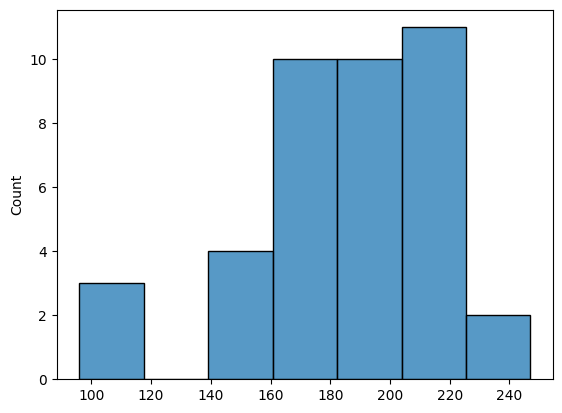
\includegraphics[width=8cm]{Histograma.png}}
    
    \subsubsection{Boxplot}  
    O Box Plot, que estudamos no curso Green Belt, é uma ferramenta gráfica que ajuda a identificar a existência de 
    possíveis outliers no conjunto de dados. Em um boxplot são apresentadas 5 estatísticas: o mínimo, o primeiro quartil 
    (Q1), a mediana, o terceiro quartil (Q3) e o máximo.
    
    \hbox{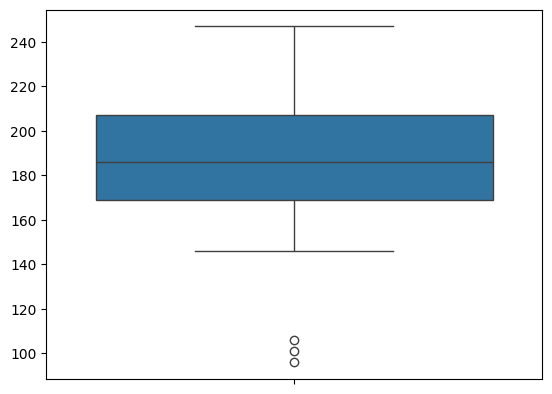
\includegraphics[width=8cm]{Boxplot.png}}   
    

  %\begin{tikzpicture}
  %  \begin{axis}
  %    \addplot3[surf, samples = 20, shader = interp]{1-x^2-y^2};
  %  \end{axis}
  % \end{tikzpicture}

\end{multicols} % Fim da seção com duas colunas
\end{document}